%% GENERATED by tools/from_docs.py from stepss-docs. Do not edit by hand:
%% edit the page named below in stepss-docs and regenerate.
%% source: stepss-docs/src/content/docs/models/exciters/stabilizers-limiters.md

\chapter{Stabilizers and limiters}\label{doc:model-exc-pss}

The power system stabilizers and over-excitation limiters that the IEEE exciter variants are combined with. They are not entered on their own: each is part of a variant such as \texttt{ST1A\_PSS2B} or \texttt{AC1A\_MAXEX2}.

The \texttt{EXC} sub-record these models are entered with, and the table of IEEE model variants, are on the \hyperref[doc:model-exc]{Exciter Models} page.

\section{PSS Models}\label{model-exc-pss:pss-models}

Power System Stabilizers (PSS) inject an additional signal \(V_{PSS}\) at the AVR summation point to damp electromechanical oscillations. All variants listed in the \hyperref[doc:model-exc]{IEEE model variants table} include one of the PSS types described here.

\subsection{PSS2B: Dual-Input Stabilizer}\label{model-exc-pss:pss2b-dual-input-stabilizer}

PSS2B accepts two input signals (typically speed \(\omega\) and electrical power \(P_e\)) and processes them through independent washout chains before combining. It corresponds to IEEE Std 421.5-2016 Type PSS2B.

\begin{docsnote}{Differences from other vendors' PSS2B}

Implementations of PSS2B vary, so parameter lists do not transfer between tools unchanged. Three differences are worth knowing when porting data in:

\begin{itemize}
\tightlist
\item
  RAMSES names the two transducer lags \(T_6\) and \(T_7\), following IEEE 421.5. Some tools name the same two constants \(T_{W6}\) and \(T_{W7}\), which is easy to misread as a third and fourth washout.
\item
  RAMSES has no \(K_{S4}\) and no ramp-tracking filter (\(AA\), \(T_A\), \(T_B\)). Data sets carrying those come from an extended PSS2B and cannot be transferred field by field.
\item
  RAMSES adds a leading \texttt{speedinput} selector that chooses the speed signal source. It has no counterpart elsewhere and must be supplied as the first stabiliser parameter.
\end{itemize}

\end{docsnote}

\[V_{S1} = \text{clamp}(VSI_1, V_{S1MIN}, V_{S1MAX})\]

Channel 1 (input 1 washout):

\[V_{S1} \xrightarrow{sT_{W1}/(1+sT_{W1})} \xrightarrow{sT_{W2}/(1+sT_{W2})} \xrightarrow{1/(1+sT_6)} pss_{3}\]

Channel 2 (input 2 washout):

\[V_{S2} \xrightarrow{sT_{W3}/(1+sT_{W3})} \xrightarrow{sT_{W4}/(1+sT_{W4})} \xrightarrow{K_{S2}/(1+sT_7)} pss_{6}\]

Combination and lead-lag chain (variant M=5, N=1 implemented):

\[pss_7 = pss_3 - K_{S3} \cdot pss_6\]

\[pss_7 \xrightarrow{(1+sT_8)/(1+sT_9)} \xrightarrow{1/(1+sT_9)^4} pss_{12}\]

\[pss_{13} = pss_{12} + pss_6\]

\[pss_{13} \xrightarrow{K_{S1}(1+sT_1)/(1+sT_2)} \xrightarrow{(1+sT_3)/(1+sT_4)} \xrightarrow{(1+sT_{10})/(1+sT_{11})} V_{PSS}\]

\[V_{PSS} = \text{clamp}(V_{PSS,unlim}, V_{STMIN}, V_{STMAX})\]

\textbf{PSS2B Parameters (additional to base exciter):}

\begin{small}\begin{longtable}[]{@{}ll@{}}
\toprule\noalign{}
Parameter & Description \\
\midrule\noalign{}
\endhead
\bottomrule\noalign{}
\endlastfoot
\texttt{speedinput} & Input selection (1=speed+power, 2=power+speed) \\
\texttt{TW1}, \texttt{TW2} & Channel 1 washout time constants \\
\texttt{T6} & Channel 1 filter \\
\texttt{TW3}, \texttt{TW4} & Channel 2 washout time constants \\
\texttt{T7}, \texttt{KS2} & Channel 2 filter gain and time constant \\
\texttt{KS3} & Channel coupling gain \\
\texttt{T8}, \texttt{T9} & Ramp-tracking filter \\
\texttt{KS1} & Overall PSS gain \\
\texttt{T1}--\texttt{T4}, \texttt{T10}, \texttt{T11} & Lead-lag time constants \\
\texttt{VS1MIN}, \texttt{VS1MAX} & Input 1 limits \\
\texttt{VS2MIN}, \texttt{VS2MAX} & Input 2 limits \\
\texttt{VSTMIN}, \texttt{VSTMAX} & Output limits \\
\end{longtable}\end{small}

\begin{center}\rule{0.5\linewidth}{0.5pt}\end{center}

\begin{figure}[htbp]
\centering
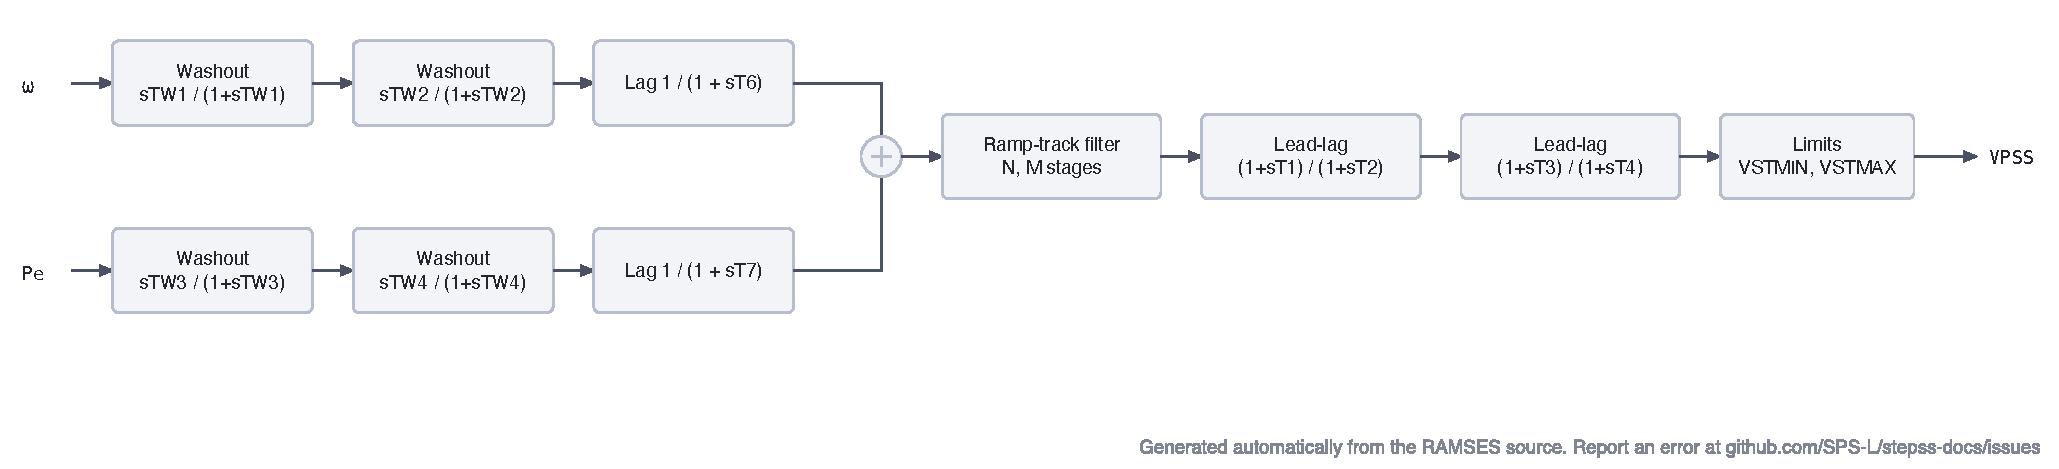
\includegraphics[width=0.98\linewidth]{figures/pss-pss2b-light}
\caption{PSS2B block diagram.}
\end{figure}

\subsection{PSS3B: Two-Input Second-Order Filter Stabilizer}\label{model-exc-pss:pss3b-two-input-second-order-filter-stabilizer}

PSS3B processes two input channels through measurement filters and washout stages, then combines them and applies two cascaded second-order lead-lag filters. It corresponds to IEEE Std 421.5-2016 Type PSS3B.

\[V_{SI1} \xrightarrow{1/(1+sT_1)} \xrightarrow{K_{S1} sT_{W1}/(1+sT_{W1})} pss_2\]

\[V_{SI2} \xrightarrow{1/(1+sT_2)} \xrightarrow{K_{S2} sT_{W2}/(1+sT_{W2})} pss_4\]

\[pss_5 = pss_2 - pss_4\]

\[pss_5 \xrightarrow{K_S sT_{W3}/(sT_{W4}+1)} pss_6\]

\[pss_6 \xrightarrow{\text{TF1: } \frac{A_2 + sA_1 + s^2/A_4}{A_4 + sA_3 + s^2/A_4}} \xrightarrow{\text{TF2: } \frac{A_6+sA_5+s^2/A_8}{A_8+sA_7+s^2/A_8}} V_{PSS}\]

\[V_{PSS} = \text{clamp}(V_{PSS,unlim}, V_{STMIN}, V_{STMAX})\]

\textbf{PSS3B Parameters (additional):}

\begin{small}\begin{longtable}[]{@{}ll@{}}
\toprule\noalign{}
Parameter & Description \\
\midrule\noalign{}
\endhead
\bottomrule\noalign{}
\endlastfoot
\texttt{speedinput} & Input mode selection \\
\texttt{T1}, \texttt{KS1}, \texttt{TW1} & Channel 1 filter, gain, washout \\
\texttt{T2}, \texttt{KS2}, \texttt{TW2} & Channel 2 filter, gain, washout \\
\texttt{KS}, \texttt{TW3}, \texttt{TW4} & Combined washout gain and time constants \\
\texttt{A1}--\texttt{A8} & Second-order filter coefficients \\
\texttt{VSTMIN}, \texttt{VSTMAX} & Output limits \\
\end{longtable}\end{small}

\begin{center}\rule{0.5\linewidth}{0.5pt}\end{center}

\begin{figure}[htbp]
\centering
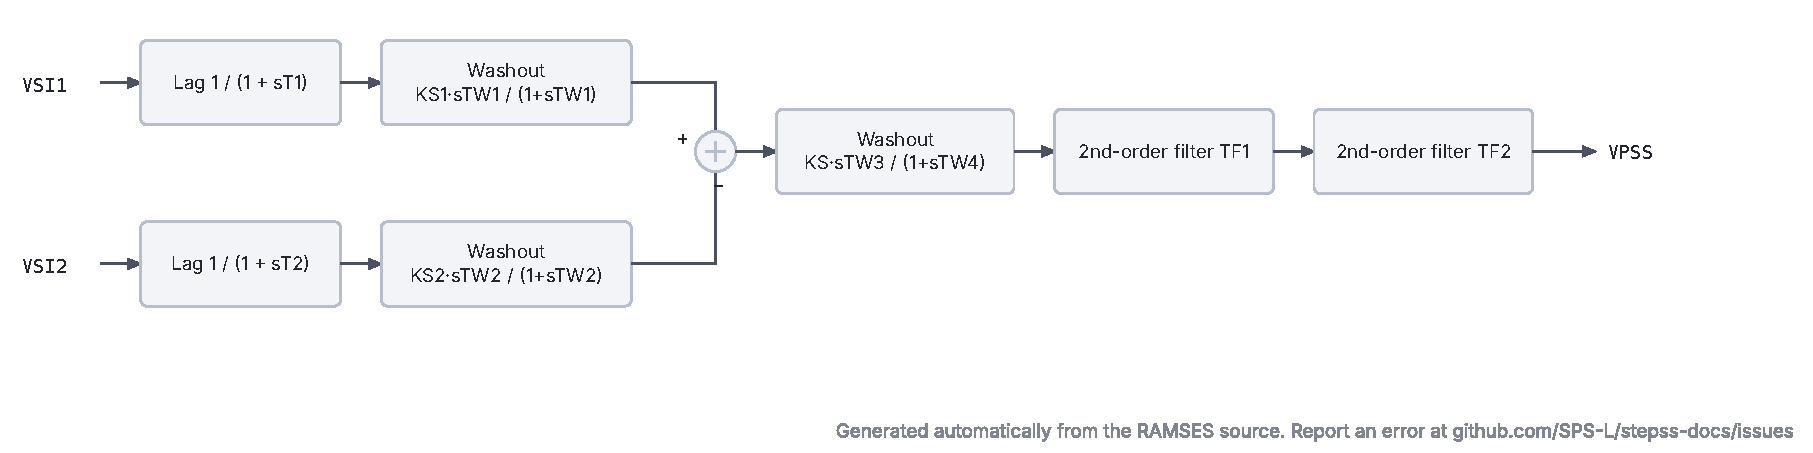
\includegraphics[width=0.98\linewidth]{figures/pss-pss3b-light}
\caption{PSS3B block diagram.}
\end{figure}

\subsection{PSS4B: Three-Band Multi-Input Stabilizer}\label{model-exc-pss:pss4b-three-band-multi-input-stabilizer}

PSS4B is a three-band stabilizer that separates the speed deviation signal into low-, intermediate-, and high-frequency components. Each band uses a pair of lead-lag filters. This model corresponds to IEEE Std 421.5-2016 Type PSS4B.

The speed signal \(\Delta\omega = \omega - 1\) passes through a digital transducer (\texttt{tf2p2z}) to obtain the low/intermediate input. Electrical power \(P_e\) passes through two washouts and a low-pass filter to derive the high-frequency component \(\Delta\omega_H\).

\textbf{Low-frequency band} (\(\Delta\omega_{L-I}\) input):

\[pss_4 = \Delta\omega_{L-I} \cdot \frac{K_{L1}(K_{L11} + sT_{L1})}{1 + sT_{L2}}\]

\[pss_5 = \Delta\omega_{L-I} \cdot \frac{K_{L2}(K_{L17} + sT_{L7})}{1 + sT_{L8}}\]

\[V_{PSSL} = \text{clamp}\!\left(K_L(pss_4 - pss_5),\, V_{LMin}, V_{LMax}\right)\]

\textbf{Intermediate-frequency band} (same \(\Delta\omega_{L-I}\) input):

\[V_{PSSI} = \text{clamp}\!\left(K_I(pss_7 - pss_8),\, V_{IMin}, V_{IMax}\right)\]

\textbf{High-frequency band} (\(\Delta\omega_H\) input):

\[V_{PSSH} = \text{clamp}\!\left(K_H(pss_{10} - pss_{11}),\, V_{HMin}, V_{HMax}\right)\]

\[V_{PSS} = \text{clamp}(V_{PSSL} + V_{PSSI} + V_{PSSH},\, V_{STMin}, V_{STMax})\]

\textbf{PSS4B Parameters (additional):}

\begin{small}\begin{longtable}[]{@{}ll@{}}
\toprule\noalign{}
Parameter & Description \\
\midrule\noalign{}
\endhead
\bottomrule\noalign{}
\endlastfoot
\texttt{H} & Generator inertia constant (for high-freq path) \\
\texttt{KL1}, \texttt{KL11}, \texttt{TL1}, \texttt{TL2} & Low-band filter 1 \\
\texttt{KL2}, \texttt{KL17}, \texttt{TL7}, \texttt{TL8} & Low-band filter 2 \\
\texttt{KL}, \texttt{VLMax}, \texttt{VLMin} & Low-band gain and limits \\
\texttt{KI1}, \texttt{KI11}, \texttt{TI1}, \texttt{TI2} & Intermediate-band filter 1 \\
\texttt{KI2}, \texttt{KI17}, \texttt{TI7}, \texttt{TI8} & Intermediate-band filter 2 \\
\texttt{KI}, \texttt{VIMax}, \texttt{VIMin} & Intermediate-band gain and limits \\
\texttt{KH1}, \texttt{KH11}, \texttt{TH1}, \texttt{TH2} & High-band filter 1 \\
\texttt{KH2}, \texttt{KH17}, \texttt{TH7}, \texttt{TH8} & High-band filter 2 \\
\texttt{KH}, \texttt{VHMax}, \texttt{VHMin} & High-band gain and limits \\
\texttt{VSTMax}, \texttt{VSTMin} & Total output limits \\
\end{longtable}\end{small}

\begin{center}\rule{0.5\linewidth}{0.5pt}\end{center}

\begin{figure}[htbp]
\centering
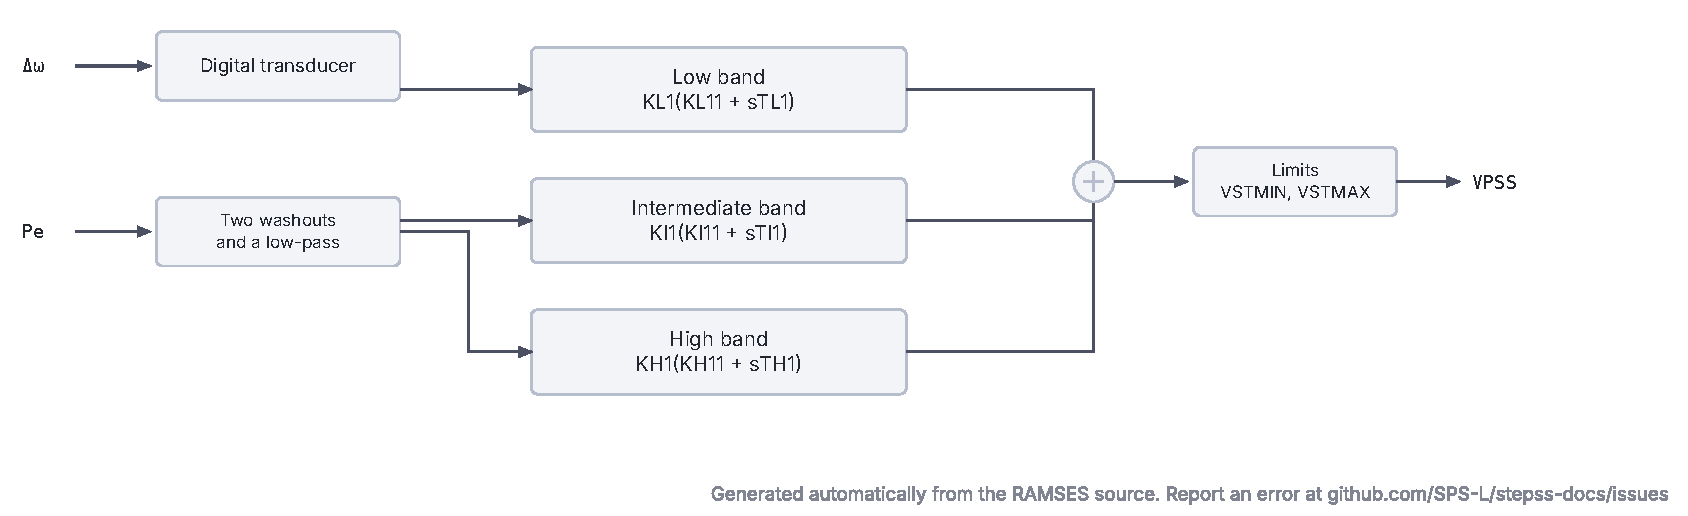
\includegraphics[width=0.98\linewidth]{figures/pss-pss4b-light}
\caption{PSS4B block diagram.}
\end{figure}

\subsection{IEEEST: Single-Input Stabilizer}\label{model-exc-pss:ieeest-single-input-stabilizer}

The IEEEST is a general-purpose single-input PSS with selectable input signal (speed deviation, electrical power, or computed accelerating power). It corresponds to IEEE Std 421.5-2016 Type PSS1A. Two second-order lead-lag filters provide frequency shaping before two first-order lead-lags and a washout stage.

\[VS_1 \xrightarrow{\frac{1}{A_2 + sA_1 + s^2/(A_1 A_2)}} \xrightarrow{\frac{A_6 + sA_5 + s^2/(A_3 A_4)}{A_4 + sA_3 + s^2/(A_3 A_4)}} VS_3\]

\[VS_3 \xrightarrow{\frac{1+sT_1}{1+sT_2}} \xrightarrow{\frac{1+sT_3}{1+sT_4}} \xrightarrow{\frac{K_S sT_5/T_6}{1+sT_6}} V_{PSS}\]

\[V_{PSS} = \text{clamp}(V_{PSS,unlim}, V_{LSMIN}, V_{LSMAX})\]

Input selection (\texttt{speedinput}): 1 = rotor speed deviation, 3 = electrical power, 4 = computed accelerating power (\(2H \, d\omega/dt\)).

\textbf{IEEEST Parameters (additional):}

\begin{small}\begin{longtable}[]{@{}ll@{}}
\toprule\noalign{}
Parameter & Description \\
\midrule\noalign{}
\endhead
\bottomrule\noalign{}
\endlastfoot
\texttt{speedinput} & Input mode (1, 3, or 4) \\
\texttt{A1}--\texttt{A6} & Second-order filter coefficients \\
\texttt{T1}--\texttt{T6} & Lead-lag and washout time constants \\
\texttt{KS} & Overall PSS gain \\
\texttt{LSMIN}, \texttt{LSMAX} & Output limits \\
\texttt{KS4} & Inertia constant for accelerating power (= 2H) \\
\texttt{TW4} & Derivative filter time constant \\
\end{longtable}\end{small}

\begin{center}\rule{0.5\linewidth}{0.5pt}\end{center}

\begin{figure}[htbp]
\centering
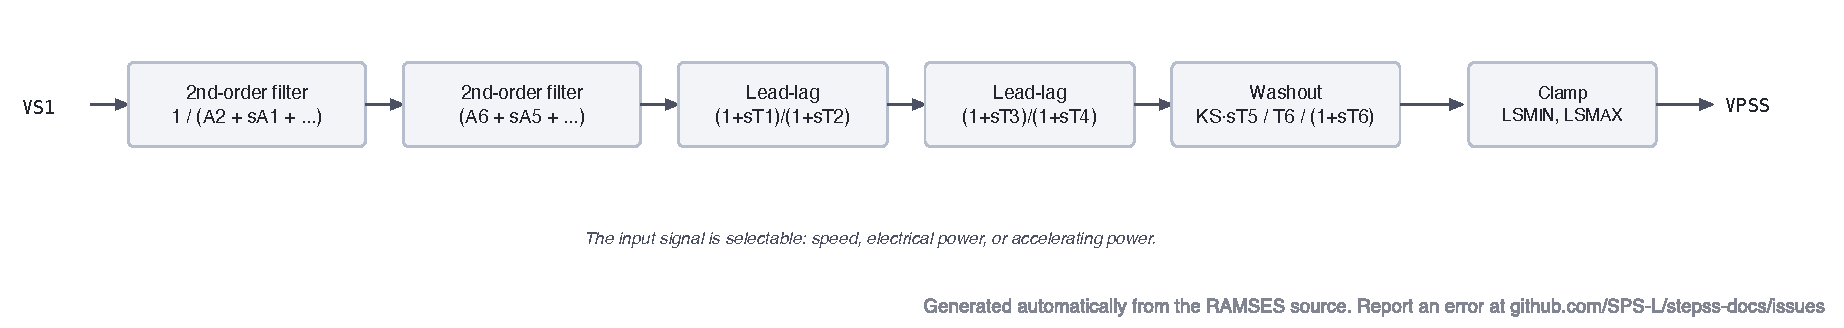
\includegraphics[width=0.98\linewidth]{figures/pss-ieeest-light}
\caption{IEEEST block diagram.}
\end{figure}

\subsection{STAB3: Power-Input Stabilizer}\label{model-exc-pss:stab3-power-input-stabilizer}

The STAB3 is a simplified PSS that takes electrical power \(P_e\) as input, applies two sequential first-order filters and a washout-type derivative block, producing a stabilizing signal.

\[P_e \xrightarrow{1/(1+sT_t)} stab_1 \xrightarrow{1/(1+sT_{X1})} stab_2 \xrightarrow{-K_X s/(1+sT_{X2})} stab_3\]

\[V_{PSS} = \text{clamp}(stab_3, -V_{LIM}, V_{LIM})\]

\textbf{STAB3 Parameters:}

\begin{small}\begin{longtable}[]{@{}ll@{}}
\toprule\noalign{}
Parameter & Description \\
\midrule\noalign{}
\endhead
\bottomrule\noalign{}
\endlastfoot
\texttt{Tt} & Input measurement time constant \\
\texttt{TX1} & First filter time constant \\
\texttt{KX} & Stabilizer gain \\
\texttt{TX2} & Washout time constant \\
\texttt{VLIM} & Output limit \\
\end{longtable}\end{small}

\begin{center}\rule{0.5\linewidth}{0.5pt}\end{center}

\section{OEL and Limiter Models}\label{model-exc-pss:oel-and-limiter-models}

Over-Excitation Limiters (OEL) prevent sustained field current overloads that would thermally damage the field winding. They generate a signal \(V_{OEL}\) that reduces the AVR output when field current exceeds thermal limits.

\begin{figure}[htbp]
\centering
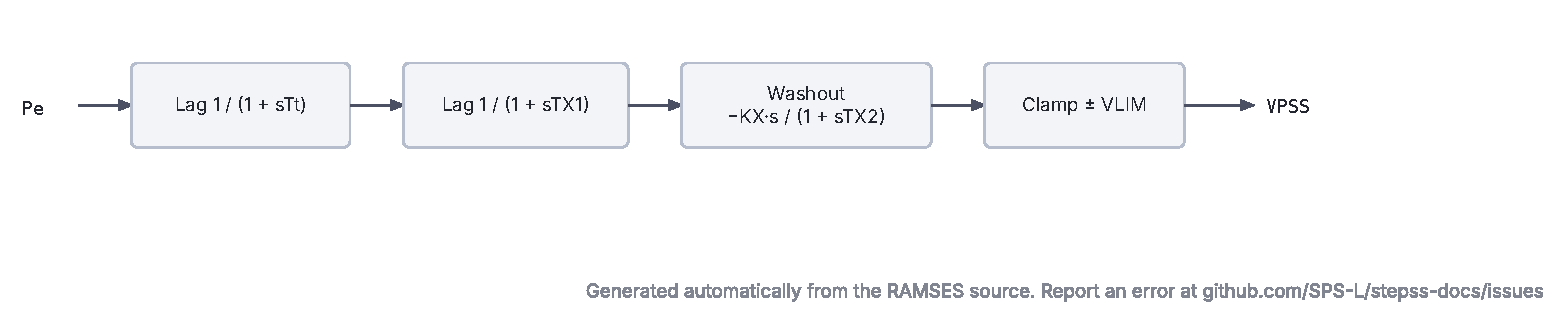
\includegraphics[width=0.98\linewidth]{figures/pss-stab3-light}
\caption{STAB3 block diagram.}
\end{figure}

\subsection{MAXEX2: Field Current Limiter with Timer and Hysteresis}\label{model-exc-pss:maxex2-field-current-limiter-with-timer-and-hysteresis}

The MAXEX2 is a field current limiter derived from IEEE work, using a simplified three-point piece-wise linear timer It is designed for the EXST1/ST1A topology where the OEL output is injected at the reference summation point (not the LV gate).

\textbf{Timer phase:} The measured current \(I_{fd,mes}\) (selected as either field current or \(E_{fd}\) via parameter \texttt{IC}) drives a \texttt{timer3} block with three \((I_{fd}, T)\) operating points. The \texttt{hyst} block latches when timer \ensuremath{\ge} 1.

\textbf{Integral phase:} Once latched, the error drives a limited integrator:

\[e_{IFD} = I_{fd,ref} - I_{fd,mes}\]

\[\dot{V}_{OEL} = \frac{e_{IFD}}{K_{MX}}, \quad V_{LOW} \le V_{OEL} \le 0\]

\(V_{OEL}\) is subtracted from the reference (\(V_{REF} - V_{OEL}\), i.e.~Negative reduces reference).

\textbf{MAXEX2 Parameters:}

\begin{small}\begin{longtable}[]{@{}ll@{}}
\toprule\noalign{}
Parameter & Description \\
\midrule\noalign{}
\endhead
\bottomrule\noalign{}
\endlastfoot
\texttt{IC} & Input selection: 0 = \(E_{fd}\), 1 = \(I_{fd}\) \\
\texttt{IFDrated} & Rated field current (reference) \\
\texttt{IFD1}, \texttt{TIME1} & Timer point 1 (current level, allowable duration) \\
\texttt{IFD2}, \texttt{TIME2} & Timer point 2 \\
\texttt{IFD3}, \texttt{TIME3} & Timer point 3 \\
\texttt{IFDDES} & Desired steady-state field current after limiting \\
\texttt{KMX} & Integrator time constant inverse (1/KMX = integration rate) \\
\texttt{VLOW} & Lower limit of OEL output (e.g.~\ensuremath{-}1.0 pu) \\
\end{longtable}\end{small}

\begin{center}\rule{0.5\linewidth}{0.5pt}\end{center}

\begin{figure}[htbp]
\centering
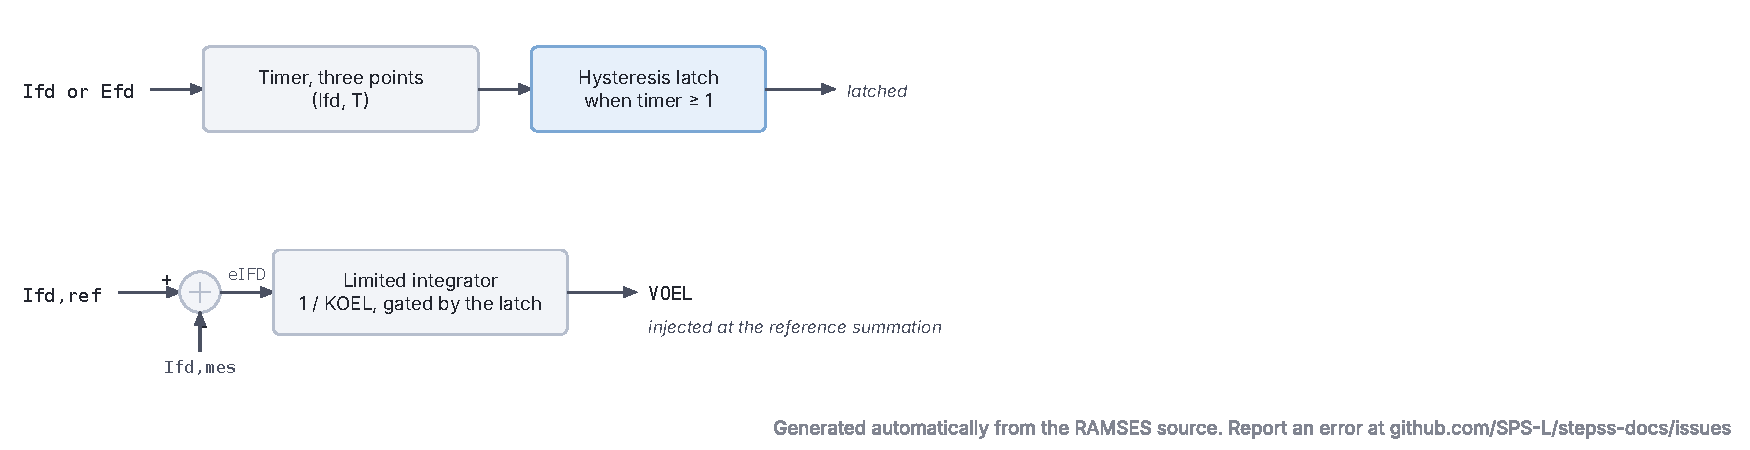
\includegraphics[width=0.98\linewidth]{figures/exc-maxex2-light}
\caption{MAXEX2 block diagram.}
\end{figure}

\subsection{Integral OEL (\_lim variants)}\label{model-exc-pss:integral-oel-_lim-variants}

The simple integral OEL used in \texttt{AC8B\_lim}, \texttt{ST1A\_lim}, \texttt{SEXS\_STAB3\_lim}, and \texttt{ENTSOE\_lim} variants computes the over-excitation signal through a clamped integrator acting on the difference between measured field current and \(1.05 \cdot I_{FDN}\), with an input clamp at \(0.35 \cdot I_{FDN}\).

\[\Delta I_{fd,1} = I_{fd} - 1.05 \cdot I_{FDN}\]

\[\Delta I_{fd,2} = \min(\Delta I_{fd,1},\, 0.35 \cdot I_{FDN})\]

\[\dot{x}_{OEL} = \frac{\Delta I_{fd,2}}{T_{OEL}}, \quad L_{OEL} \le x_{OEL} \le U_{OEL}\]

\[V_{OEL} = \text{clamp}(K_{OEL} \cdot x_{OEL},\, OEL_{LI},\, 0)\]

A stator current limiter (SCL) with analogous structure acts on \(I_{st} = \sqrt{P^2 + Q^2}/V_t\) relative to \(1.025 \cdot I_{GN}\).

\textbf{Integral OEL Parameters (in \_lim variants):}

\begin{small}\begin{longtable}[]{@{}ll@{}}
\toprule\noalign{}
Parameter & Description \\
\midrule\noalign{}
\endhead
\bottomrule\noalign{}
\endlastfoot
\texttt{IFDN} & Nominal field current (OEL trigger at 1.05\ensuremath{\times}) \\
\texttt{TOEL} & OEL integrator time constant \\
\texttt{LOEL} & OEL integrator lower limit \\
\texttt{UOEL} & OEL integrator upper limit \\
\texttt{KOEL} & OEL output gain \\
\texttt{OELLI} & OEL output lower limit \\
\texttt{IGN} & Nominal stator current (SCL trigger at 1.025\ensuremath{\times}) \\
\texttt{TSCL} & SCL integrator time constant \\
\texttt{LSCL} & SCL integrator lower limit \\
\texttt{USCL} & SCL integrator upper limit \\
\texttt{KSCL} & SCL output gain \\
\texttt{SCLLI} & SCL output lower limit \\
\end{longtable}\end{small}

\begin{center}\rule{0.5\linewidth}{0.5pt}\end{center}

For full documentation of the CODEGEN DSL primitives used in these models (\texttt{tf1p}, \texttt{tf1p1z}, \texttt{tf1plim}, \texttt{inlim}, \texttt{pictl}, etc.), see the \hyperref[ch-libray_blocks]{CODEGEN Blocks} reference.

\begin{figure}[htbp]
\centering
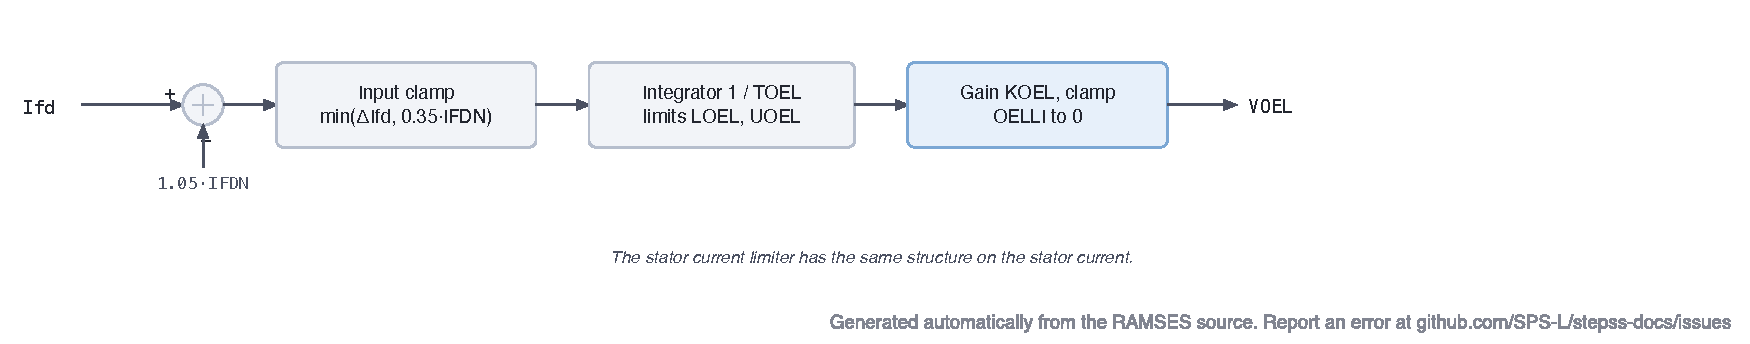
\includegraphics[width=0.98\linewidth]{figures/exc-integral-oel-light}
\caption{Integral over-excitation limiter block diagram.}
\end{figure}
